\newcommand{\U}[1]{\ensuremath{\,\textrm{#1}}}
\newcommand{\tref}{\ensuremath{\textrm{ref}}}
\newcommand{\vthref}{\ensuremath{v_\textrm{thref}}}
\newcommand{\gkw}{\ensuremath{\textrm{GKW}}}
\newcommand{\gkdb}{\ensuremath{\textrm{GKDB}}}

\documentclass[a4paper]{report}
\usepackage{fullpage}
\usepackage{amsmath}
\usepackage{amssymb}
\usepackage{bm}
\usepackage{graphicx}
\usepackage{tabularx}
\usepackage{hyperref}

\hypersetup{bookmarks, plainpages=false, colorlinks=true, pdfborder={0 0 0 0}, linkcolor=blue, citecolor=blue, urlcolor=blue, pdftitle={GKDB documentation}}

\begin{document}

\title{Documentation of the GKW to GKDB data conversion}

\author{Y. Camenen on behalf of the GKDB working group}

\date{Last update: February 9, 2018}

\maketitle

\chapter{Preface}
This document describes how to transform inputs and outputs from a GKW flux-tube simulation to match the format used in the GyroKinetic DataBase (GKDB).  
The reader is assumed to have some knowledge of GKW and to have read the documentation of the GKDB.

\tableofcontents

\chapter{Conventions and normalisations}

\section{Coordinate systems}

In GKW, the toroidal direction is defined to have the cylindrical coordinate system $(R,Z,\varphi)$ right-handed whereas in the GKDB it is defined to have $(R,\varphi,Z)$ right-handed, see Fig.\ref{fig:coord1}. In practice, it means that: 
\begin{equation}
\varphi^\gkw=-\varphi^\gkdb
\end{equation}
\begin{figure}[h]
	\begin{center}
		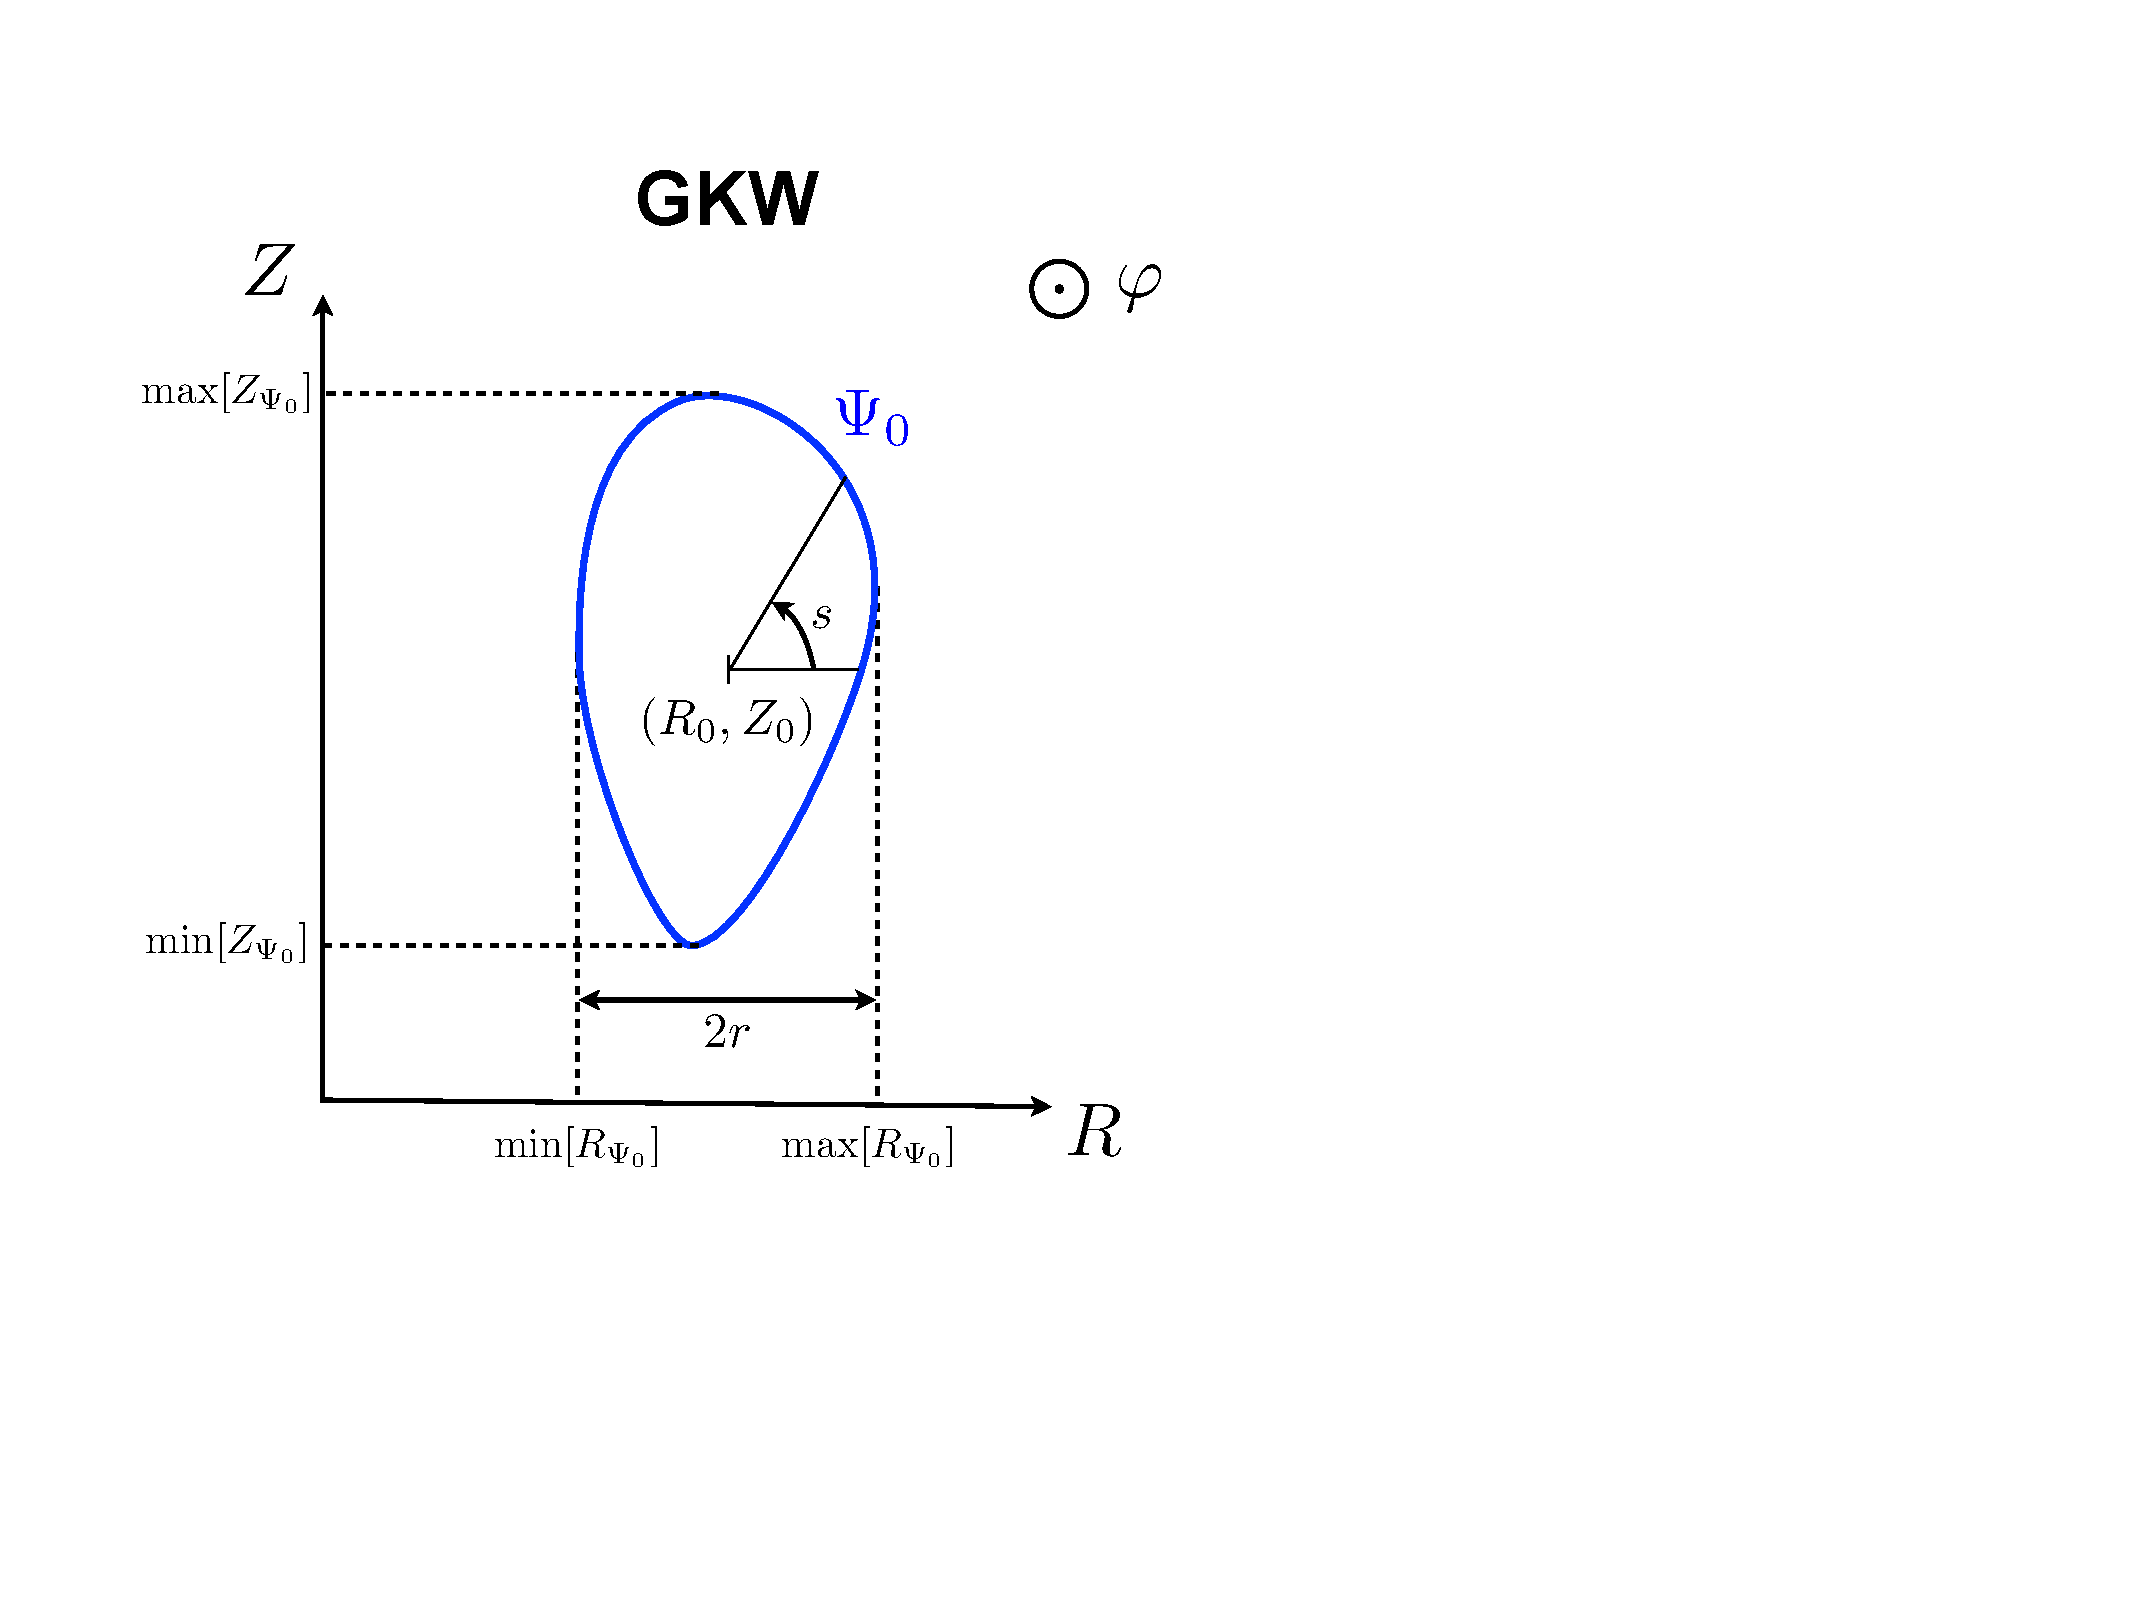
\includegraphics[width=7cm]{GKW_coord.pdf}
		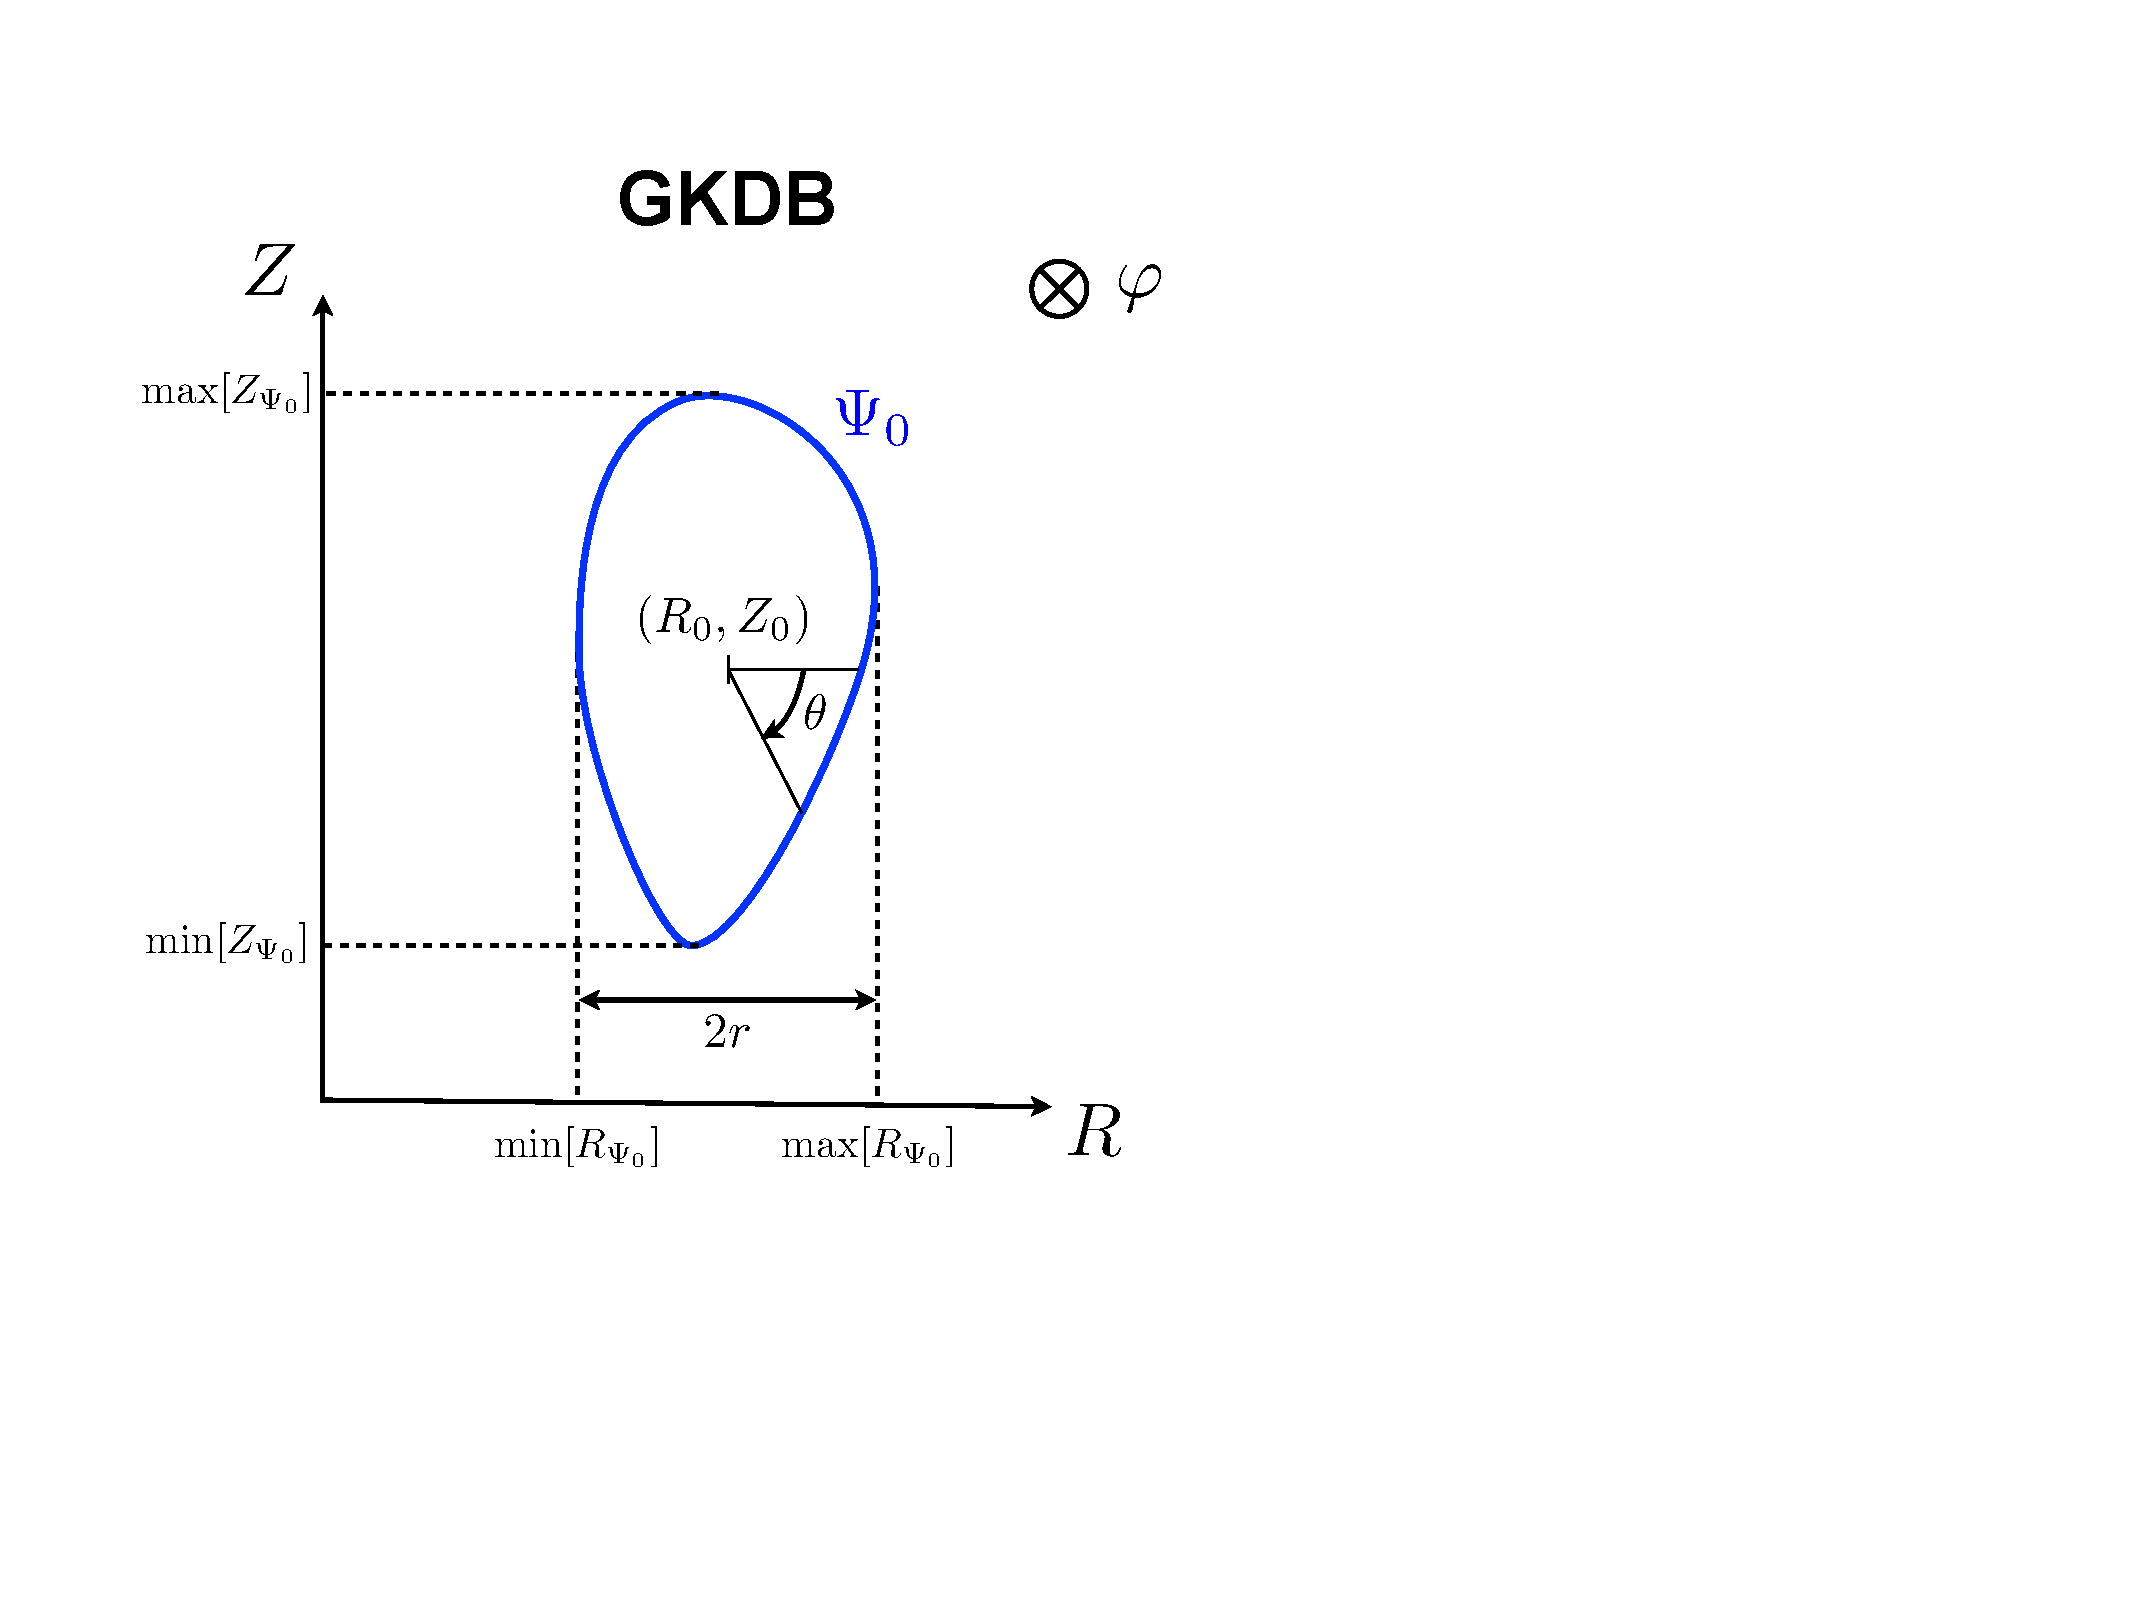
\includegraphics[width=7cm]{GKDB_coord.pdf}
		\caption{\label{fig:coord1} Cylindrical coordinate system used in GKW (left) and the GKDB (right).}
	\end{center}
\end{figure}\\
The flux surface centre definition depends on how the magnetic equilibrium is specified. For \texttt{miller} geometry, the definition of $R_0$ is identical to that used in the GKDB and $Z_0$ is given as an input in the geometry namelist:
\begin{equation}
R_0^\texttt{GKW-miller} = R_0^\gkdb \qquad \qquad Z_0^\texttt{GKW-miller} = \texttt{zmil}R_\tref^\gkw
\end{equation}
For \texttt{chease} geometry, $R_0$ is taken to be the value of \texttt{R0EXP} specified in the \texttt{hamada.dat} file and $Z_0$ is the elevation of the magnetic axis.
\begin{equation}
R_0^\texttt{GKW-chease} = \texttt{R0EXP} \qquad \qquad Z_0^\texttt{GKW-chease} = Z_\textrm{axis}
\end{equation}
The definition of the (unnormalised) radial coordinate $r$ is identical in GKW and the GKDB:
\begin{equation}
r^\gkw = r^\gkdb
\end{equation}
The calculation of the GKDB poloidal angle $\theta$ from GKW inputs is documented in section~\ref{sec:magequil}. At this stage, just notice that as  $Z_0^\gkw\neq Z_0^\gkdb$ the points $s=0$ and $\theta=0$ do not  coincide. 


\section{Reference quantities}


\chapter{Inputs}
\section{Magnetic equilibrium} \label{sec:magequil}
Only \texttt{miller} and \texttt{chease} magnetic equilibrium specifications are compatible with the GKDB format. 


\chapter{Outputs}

\bibliographystyle{unsrt}
\bibliography{gkw2gkdb}

\end{document}
